%\documentclass[table, 10pt]{beamer}%
\documentclass[table, 10 pt, handout]{beamer}%

\usepackage[french]{babel}
\usepackage{tikz}
\usepackage[latin1]{inputenc}
\usepackage{times}
\usepackage[T1]{fontenc}

\usepackage{graphicx,graphics}

\usepackage{amsmath,amsfonts}

\usepackage{multirow}

%\usepackage[table]{xcolor}

%\usepackage{beamerthemeliris}

\usepackage{beamerthemesplit}
\usetheme{Malmoe}%Copenhagen%Dresden%Malmoe
\usecolortheme{orchid}%beetle,seagull,crane,dove,orchid
\useinnertheme[shadow]{rounded}%rounded
\usefonttheme{professionalfonts}

\definecolor{darkgreen}{RGB}{0,180,0} 

\setbeamertemplate{navigation symbols}{}


\newenvironment{codeblock}[1]{\begin{exampleblock}<+->{\texttt{#1}}\begin{tt}}{\end{tt}\end{exampleblock}}




\title[S21 - Comprendre les r�seaux -- CM \hspace{1cm}\insertframenumber{} / \inserttotalframenumber]
{S21 -- Comprendre les r�seaux }
\subtitle{CM}
\author[Julien Gossa]{Julien Gossa}
\institute
{ 
	{\bf IUT Robert Schuman -- D�partement Informatique}\\
	{\url{julien.gossa@unistra.fr}}
}

\date{2009}
\beamertemplatetransparentcovereddynamicmedium 

\begin{document}


\begin{frame}
 	\titlepage
\end{frame}



\AtBeginSection[]
{
   \begin{frame}
       \frametitle{Sans transition\ldots}
       %\small
       \tableofcontents[currentsubsection]
   \end{frame}
}	

\AtBeginSubsection[]
{
   \begin{frame}
       \frametitle{Sans transition\ldots}
       %\small
       \tableofcontents[currentsubsection]
   \end{frame}
}	

% ----------------------------------------------------------------------
\section{Mod�le OSI}
% ----------------------------------------------------------------------
\begin{frame}
	\begin{columns}
	
	\column{0.5\textwidth}
		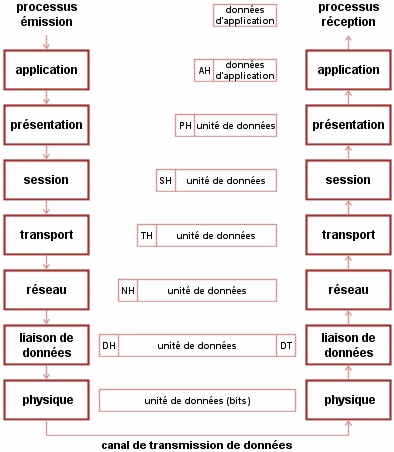
\includegraphics[width=\textwidth]{res/osi_com}
	
	\column{0.5\textwidth}
		\begin{block}<+-> {Mod�le OSI}
			\begin{itemize}
				\item S�paration en couches
				\item Chacune rend un service � celle juste au dessus
				\item Les donn�es doivent traverser toutes les couches
				\item Avantages :
				\begin{itemize}
					\item R�duit la complexit�
					\item Uniformise les interfaces
					\item Assure l'interop�rabilit�
					\item Facilite la conception modulaire
					\item Acc�l�re l'�volution
				\end{itemize}
			\end{itemize}
		\end{block}
		
	\end{columns}


\end{frame}
% ----------------------------------------------------------------------


% ----------------------------------------------------------------------
\begin{frame}
	\begin{columns}
	
	\column{0.5\textwidth}
		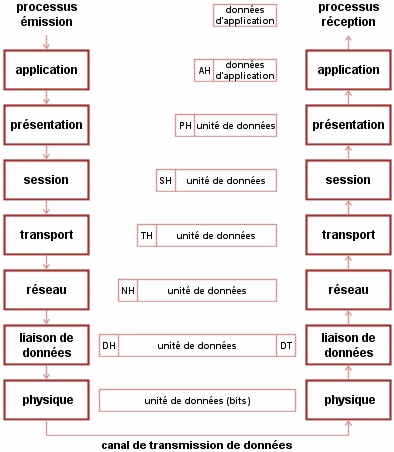
\includegraphics[width=\textwidth]{res/osi_com}
	
	\column{0.5\textwidth}
		\begin{block}<+-> {1. couche physique}
			\begin{itemize}
				\item Transmission des signaux
				\item Entre deux interlocuteurs
				\item Emission/R�ception de bits
				\item = C�ble
			\end{itemize}
		\end{block}
		
	\end{columns}

\end{frame}
% ----------------------------------------------------------------------

% ----------------------------------------------------------------------
\begin{frame}
	\begin{columns}
	
	\column{0.5\textwidth}
		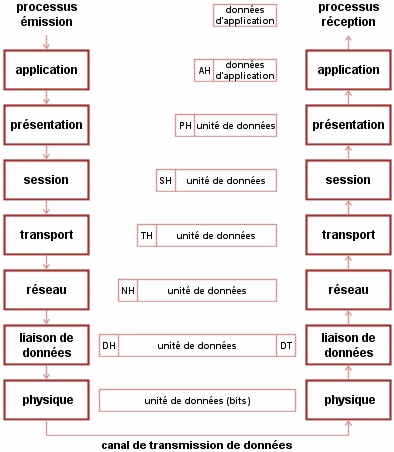
\includegraphics[width=\textwidth]{res/osi_com}
	
	\column{0.5\textwidth}
		\begin{block}<+-> {2. couche liaison de donn�es}
			\begin{itemize}
				\item Communications
				\item Entre deux machines adjacentes
				\item Dans LAN 
				\item Protocole Ethernet
				\item Ajout adresse MAC
				\item Switch, Hub
			\end{itemize}
		\end{block}
		
	\end{columns}

\end{frame}
% ----------------------------------------------------------------------

% ----------------------------------------------------------------------
\begin{frame}
	\begin{columns}
	
	\column{0.5\textwidth}
		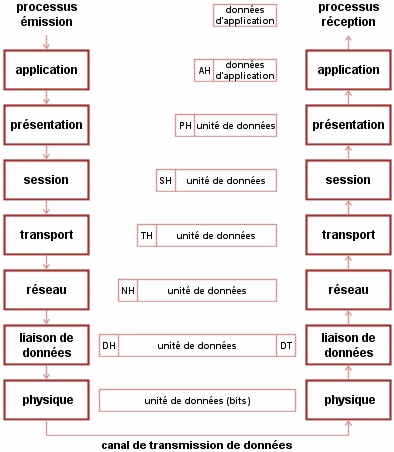
\includegraphics[width=\textwidth]{res/osi_com}
	
	\column{0.5\textwidth}
		\begin{block}<+-> {3. couche r�seau}
			\begin{itemize}
				\item Communications
				\item De proche en proche
				\item Routage / Adressage
				\item Protocole IP
				\item Routeur
			\end{itemize}
		\end{block}
		
	\end{columns}

\end{frame}
% ----------------------------------------------------------------------

% ----------------------------------------------------------------------
\begin{frame}
	\begin{columns}
	
	\column{0.5\textwidth}
		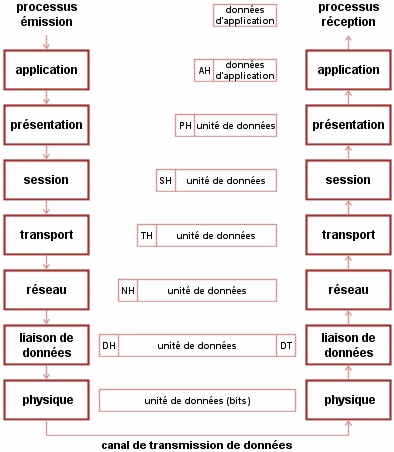
\includegraphics[width=\textwidth]{res/osi_com}
	
	\column{0.5\textwidth}
		\begin{block}<+-> {4. Couche transport}
			\begin{itemize}
				\item Communications
				\item Entre processus
				\item Socket, ports
				\item Protocoles TCP, UDP, ICMP
				\item Pare-feu, NAT
			\end{itemize}
		\end{block}
		
	\end{columns}

\end{frame}
% ----------------------------------------------------------------------

% ----------------------------------------------------------------------
\begin{frame}
	\begin{columns}
	
	\column{0.5\textwidth}
		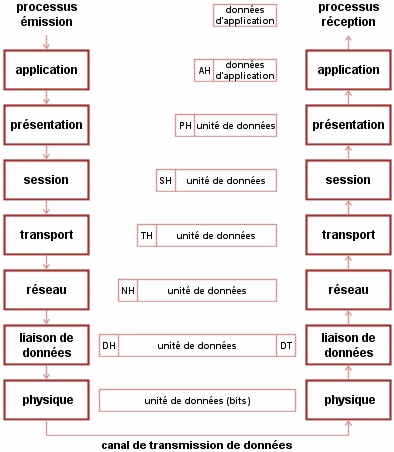
\includegraphics[width=\textwidth]{res/osi_com}
	
	\column{0.5\textwidth}
		\begin{block}<+-> {5. Couche session}
			\begin{itemize}
				\item Synchronisation et Transaction
				\item Mal support� par IP
			\end{itemize}
		\end{block}
		
	\end{columns}

\end{frame}
% ----------------------------------------------------------------------


% ----------------------------------------------------------------------
\begin{frame}
	\begin{columns}
	
	\column{0.5\textwidth}
		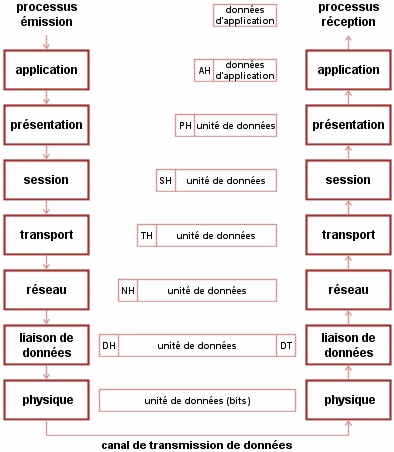
\includegraphics[width=\textwidth]{res/osi_com}
	
	\column{0.5\textwidth}
		\begin{block}<+-> {6. Couche pr�sentation}
			\begin{itemize}
				\item Codage
				\item Des Donn�es applicatives
				\item Pour transmission
				\item ASCII, Unicode, HTML
			\end{itemize}
		\end{block}
		
	\end{columns}

\end{frame}
% ----------------------------------------------------------------------

% ----------------------------------------------------------------------
\begin{frame}
	\begin{columns}
	
	\column{0.5\textwidth}
		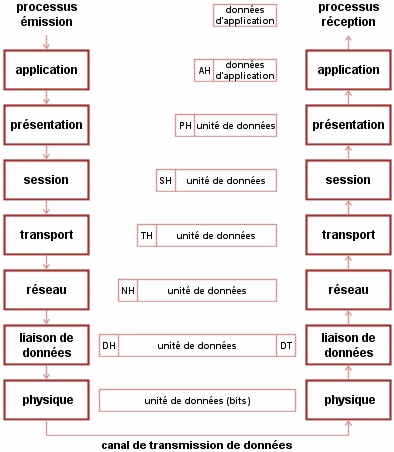
\includegraphics[width=\textwidth]{res/osi_com}
	
	\column{0.5\textwidth}
		\begin{block}<+-> {7. Couche applicative}
			\begin{itemize}
				\item Points d'acc�s
				\item Aux services r�seaux
				\item SSH, SMTP, POP3, IMAP, HTTP, FTP
			\end{itemize}
		\end{block}
		
	\end{columns}

\end{frame}
% ----------------------------------------------------------------------

\begin{frame}{Conclusion}
\tableofcontents
\end{frame}

\end{document}